
%we experiment with the dataset proposed by \cite{luo2016temporal} which aims at extracting relations between entity and time. With some heuristics, this dataset can be further split intro three subsets with different levels of reliability, which enables us to conduct all our experiment settings. To show the generalization ability of our model, we also experiment with the dataset proposed by \cite{riedel2010modeling}, which aims at extracting relations between entities and there is no prior knowledge of the data quality can be used. \todo{can be shorter}

%We also consider two types of relation extraction tasks. The first task aims at extracting relations between entity and time. Specifically, it requires the object to be an time expression and the subject to be an entity. As suggested by \cite{luo2016temporal}, the distant supervision dataset in this task can be naturally divided into several subsets with different levels of reliability. The basic idea is that number of important things related to one entity increases as the time scope becomes larger. For example, a sentence containing both \emph{Alphabet} and \emph{October\_2\_2015} is very likely to express the foundation time of \emph{Alphabet}, while a sentence containing both \emph{Alphabet} and \emph{2015} may instead talk about its financial report of year 2015. We experiment with this task because it has a public dataset that contains both reliable and unreliable data, which enables us to conduct all of our experiments.

%The second task aims at extracting relations between entities, which is extensively studied in relation extraction. We experiment with this task to see if our transition matrix method generalizes well in different datasets.

\begin{figure}[t!]
\begin{center}
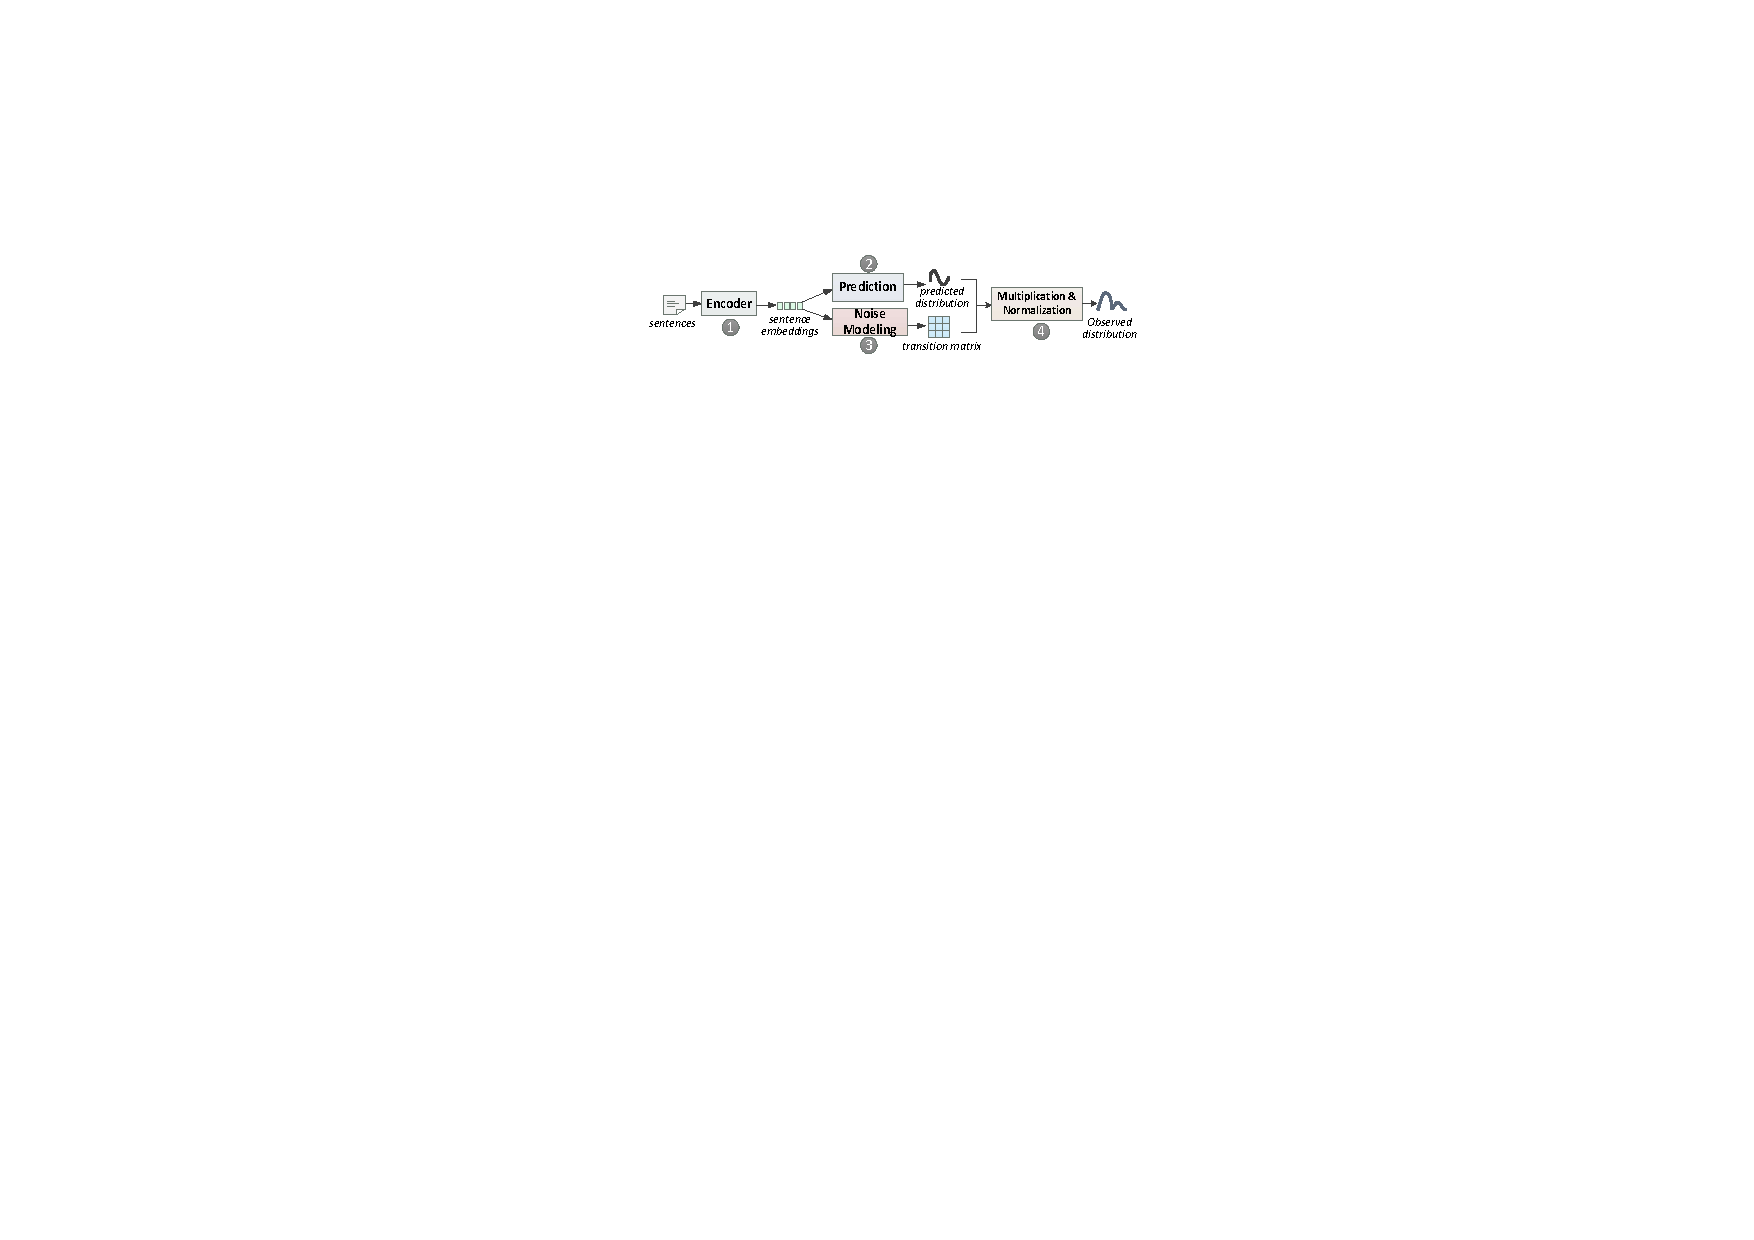
\includegraphics[width=0.5\textwidth]{figures/overview.pdf}	
\caption{Overview of our approach}
\label{fig: denoise_framework}
\end{center}
\end{figure}


\section{Our approach}
%Our approach for distantly supervised relation extraction is depicted in Figure \ref{fig: denoise_framework}.
%First, the input sentence (or sentence
%bag) is passed to a sentence encoder to get sentence embedding(s). After that, the model is split into two branches.
%The prediction branch generates the predicted relation distribution $\mathbf{p}$ of the input sentence (or sentence
%bag). The noise modeling branch generates the transition matrix $\mathbf{T}$. Finally, the predicted distribution is
%multiplied by the transition distribution to generate the observed relation distribution $\mathbf{o}$. The predicted
%relation distribution $\mathbf{p}$ is the output of the model while the observed relation distribution $\mathbf{o}$ is
%used to simulate the relation assigned by distant supervision. In this way, the noise is modeled by the transition
%matrix and the real
%prediction is protected from the influence of the noise. In rest of this section, we will first describe the sentence level model, and then extend the model to bag level.
%
%\subsection{Sentence Encoder}
%The sentence encoder serves to transform an input sentence to an embedding vector that encodes semantic meaning of the sentence. Theoretically, almost any sentence encoder would work here. Similar to previous researches, we also use the piecewise convolutional neural network (PCNN) model \cite{zeng2015distant} as our sentence encoder. First, the distances of each word to the subject and the object are embedded as randomly initialized vectors and concatenated to the original word vector. After that, the PCNN model divides the input sentence into three pieces by the subject and the object, and apply convolutional neural network (CNN) to each piece to calculate the piece embedding. The final sentence embedding is the concatenation of the embeddings of the three pieces.

To model the noise distribution of relations, our approach follows four steps as depicted in Figure \ref{fig: denoise_framework}.
First, each input sentence is parsed by a sentence encoder to generate an embedding vector. In this work, we
use a piecewise convolutional neural network~\cite{zeng2015distant} for sentence encoding, but other encoding models can also be
used. After encoding, our model takes in the sentence embeddings to generate a predicted relation
distribution, $\mathbf{p}$, for the input sentence (or sentence bag). The model also generates a transition matrix,
$\mathbf{T}$, which is used to model the noise of the \DS-generated relations. Finally, the predicted distribution is
multiplied by the transition matrix to produce the observed relation distribution, $\mathbf{o}$. The predicted
relation distribution $\mathbf{p}$ is the output of our model while the observed relation distribution $\mathbf{o}$ is
used to capture the relation assigned by \DS. 


One of the key challenges of our approach is
on determining the weights of the transition matrix, $\mathbf{T}$. This is described in Section~\ref{sec:training}.
In the remainder of this section, we will describe how our approach can be
applied to sentence- and bag-level models. 



\subsection{Prediction Branch}
The prediction branch generates the predicted relation distribution $\mathbf{p}$ and can be implemented by the
prediction part of almost any relation extraction neural network models. Similar to \cite{luo2016temporal}, for
sentence level models, we first feed the sentence embedding to a full connection layer, and then use softmax for
relation classification.
\todo{ZW: I assume this is not a new contribution?}

\subsection{Noise Modeling Branch}
The noise modeling branch calculates a transition matrix dynamically for each sentence (or sentence bag) to model its noise pattern.

For sentence level models, the sentence embedding $\mathbf{x}$ is passed to another full connection layer to obtain the sentence embedding $\mathbf{x}_n$ used specifically for noise modeling branch. The transition matrix $\mathbf{T}$ is calculated using softmax function :
\begin{equation}
T_{ij} = \frac{exp({\mathbf{w}_{ij}^T \mathbf{x}_n + b})}{\sum_{j=1}^{|\mathbb{C}|}{exp({\mathbf{w}_{ij}^T \mathbf{x}_n + b}})}
\end{equation}
where $T_{ij}$ is the conditional probability that this sentence is labeled as relation $j$ by distant supervision given $i$ as the true relation, $\mathbf{w}_{ij}$ is the weight vector for this situation, $b$ is a scalar bias and $|\mathbb{C}|$ is the number of relations. Note that the softmax function guarantees that each row of the transition matrix $\mathbf{T}$ sums to 1.

\subsection{Observed Relation Distribution}
The observed relation distribution $\mathbf{o}$ is calculated by multiplying transition matrix $T$ and the predicted relation distribution $p$:
 \begin{equation}
\mathbf{o} = \mathbf{T}^T \bm\cdot \mathbf{p}
\label{eq_transition}
 \end{equation}
 \iffalse
 \begin{equation}
 \label{norm_o}
 o_i = \frac{o_i}{\sum_i{o_i}}
 \end{equation}
 \fi
 where $\bm\cdot$ represents dot product and we normalizes the elements of $\mathbf{o}$ so that $\sum_i{o_i}=1$ afterwards.

Different from previous works that use the predicted relation distribution $\mathbf{p}$ to directly match the relation labeled by distant supervision. \orange{We instead use $\mathbf{o}$ to match the noisy label and still use $\mathbf{p}$ as output}. Note that if the true relation of the input training instance is $i$, we can assume that this relation $i$ could be labeled as relation $j$ by distant supervision with probability $T_{ij}$. Therefore, Equation \ref{eq_transition} actually models the procedure of how the noisy label is produced and thus \orange{protects $\mathbf{p}$ from the bad influence of noise.}
%can help the model make better use of the noisy training data. \red{How to better use?? by using regularization????}

Also note that the noise modeling branch and $\mathbf{o}$ is only used in the training phase. In the test phase, we only use the prediction brach and take the predicted relation distribution $\mathbf{p}$ as our output. \todo{last paragraph can be removed}

\subsection{Bag Level Models}
\paragraph{Bag Level Prediction Branch}
The key problem in the bag level prediction branch is how to aggregate the embeddings of each sentence in the bag. Here we experiment with two methods, average and attention aggregation. The average aggregation calculates the bag embedding $\mathbf{s}$ by averaging the embeddings of each sentence, and the resultant bag embedding is fed to a softmax classifier for relation classification.

The attention aggregation method is proposed by \cite{lin2016neural}. It calculates an attention value for each sentence with respect to each relation, and uses the following equation to calculate the bag embedding with respect to relation $j$:
\begin{equation}
\mathbf{s}_j = \sum_i^{n}{\alpha_{ij} \mathbf{x}_{i}}
\label{eq_att_bag_embed}
\end{equation}
where $\mathbf{x}_{i}$ is the embedding of sentence $i$, $n$ is the number of sentences in the bag and $\alpha_{ij}$ is the attention value over sentence $i$ with respect to relation $j$. The resultant bag embedding is fed to a softmax classifier to predict the probability of relation $j$.

\paragraph{Bag Level Transition Matrix}
\orange{We use attention mechanism to generate transition matrix for both average and attention aggregation models.} Specifically, we calculate the bag embedding with respect to each relation with Equation \ref{eq_att_bag_embed}, and the attention value for sentence $i$ with respect to relation $j$ is calculated by:
\begin{equation}
\alpha_{ij} = \frac{exp(\mathbf{x}_i^T \mathbf{r}_t^j)}{\sum_i^n{exp(\mathbf{x}_i^T \mathbf{r}_t^j)}}
\end{equation}
where $\mathbf{x}_i$ is the embedding of sentence $i$ and $\mathbf{r}_t^j$ is the randomly initialized embedding of relation $j$ used specifically for noise modeling branch.

Then the transition matrix $\mathbf{T}$ is calculated by:
\begin{equation}
T_{ij} = \frac{exp({\mathbf{s}_i^T \mathbf{r}_t^j  + b})}{\sum_{j=1}^{|\mathbb{C}|}{exp(\mathbf{s}_i^T \mathbf{r}_t^j + b})}
\end{equation}
where $\mathbf{s}_i$ is the bag embedding with respect to relation $i$, $\mathbf{r}_t^j$ is the same embedding of relation $j$.


